\documentclass[11pt]{article}

\usepackage{amsmath}
\usepackage{amssymb}
\usepackage{graphicx}
\usepackage{caption}
\usepackage{subcaption}

\topmargin -.5in
\textheight 9in
\oddsidemargin -.25in
\evensidemargin -.25in
\textwidth 7in

\newcommand{\code}[1]{\texttt{#1}}

\begin{document}

\author{Gu, Qiao}
\title{16-720B Homework 2 Write-up}
\maketitle

\medskip

\subsection*{Q1.2}

Please see Figure.~\ref{fig:q1.2} for the DoG Pyramid of \code{model\_chickenbroth.jpg}.

\begin{figure}[h!]
    \centering
    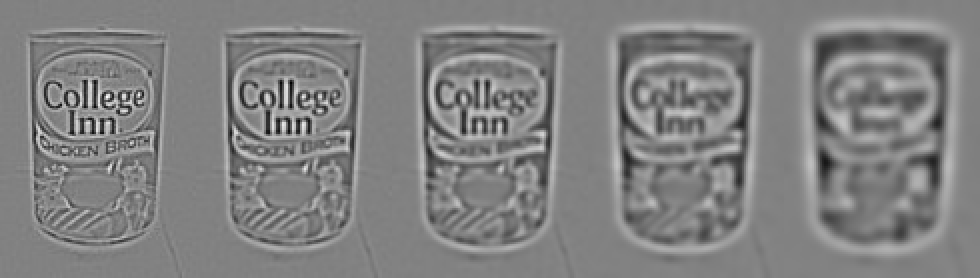
\includegraphics[width=.8\linewidth]{../results/q1_2.png}
    \caption{The DoG Pyramid of \code{model\_chickenbroth.jpg}}
    \label{fig:q1.2}
\end{figure}

\newpage

\subsection*{Q1.5}

Please see Figure.~\ref{fig:q1.5} for the detected keypoints of \code{model\_chickenbroth.jpg}.

\begin{figure}[h!]
    \centering
    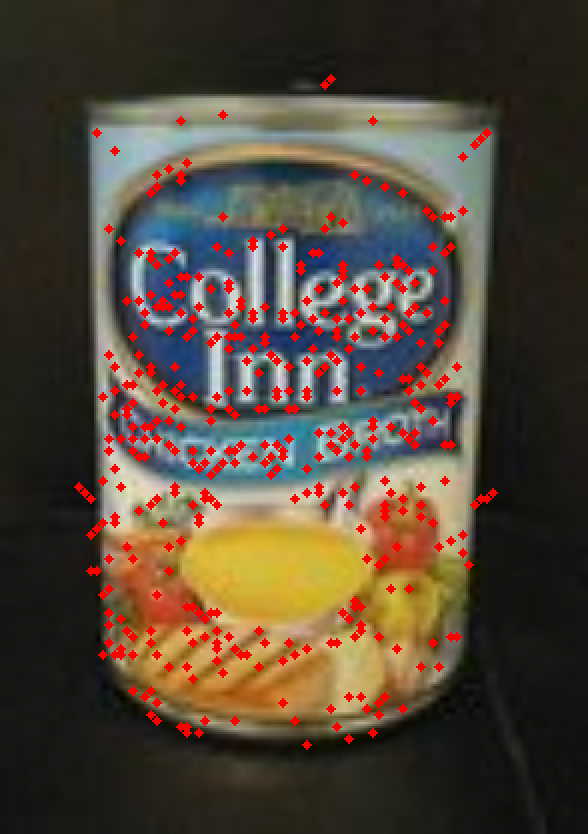
\includegraphics[width=.4\linewidth]{../results/q1_5.png}
    \caption{The detected keypoints on image \code{model\_chickenbroth.jpg}}
    \label{fig:q1.5}
\end{figure}

\newpage

\subsection*{Q2.4}

Please see Figure~\ref{fig:q2.4} for the matching results. From the results, we can see that if the object is rotated, the matching performance will be much worse than those with little or no rotation (compare Figure.~\ref{fig:q2.4} (d)(g) with Figure.~\ref{fig:q2.4} (c)(f)). I suspect this is because the BRIEF descriptor does not encode the patch into a rotation-invariant space and thus have poor ability to match rotated patches.

\begin{figure}[h!] \label{fig:q2.4}
    \begin{subfigure}{.49\textwidth}
      \centering
      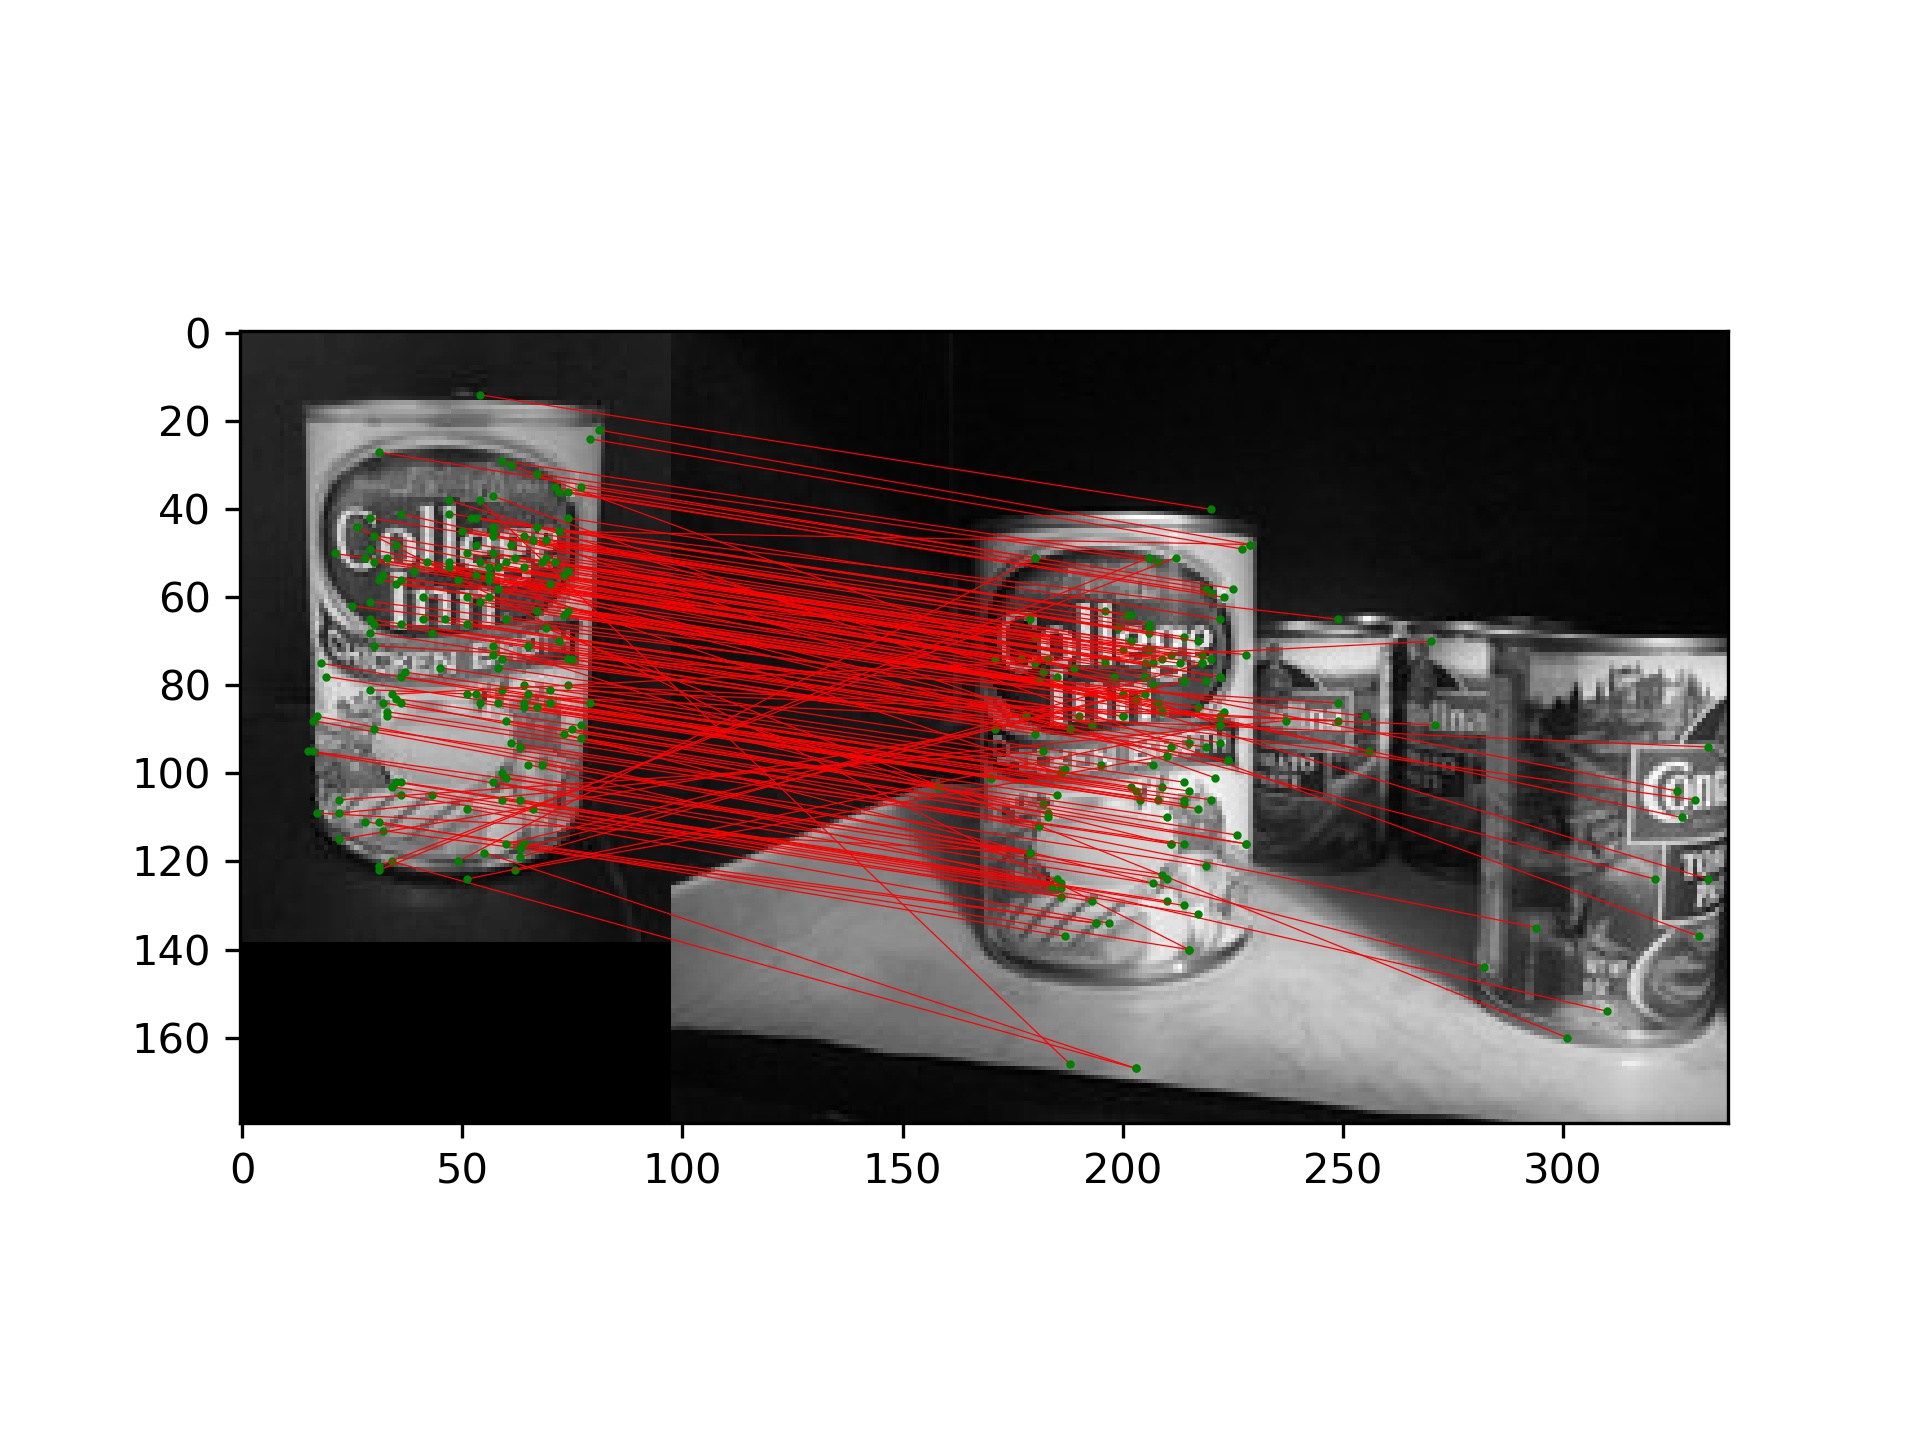
\includegraphics[width=.8\linewidth]{../results/chickenbroth_01_match.jpg}
      \caption{match of two of the \code{chickenbroth} images.}
    \end{subfigure}
    \begin{subfigure}{.49\textwidth}
      \centering
      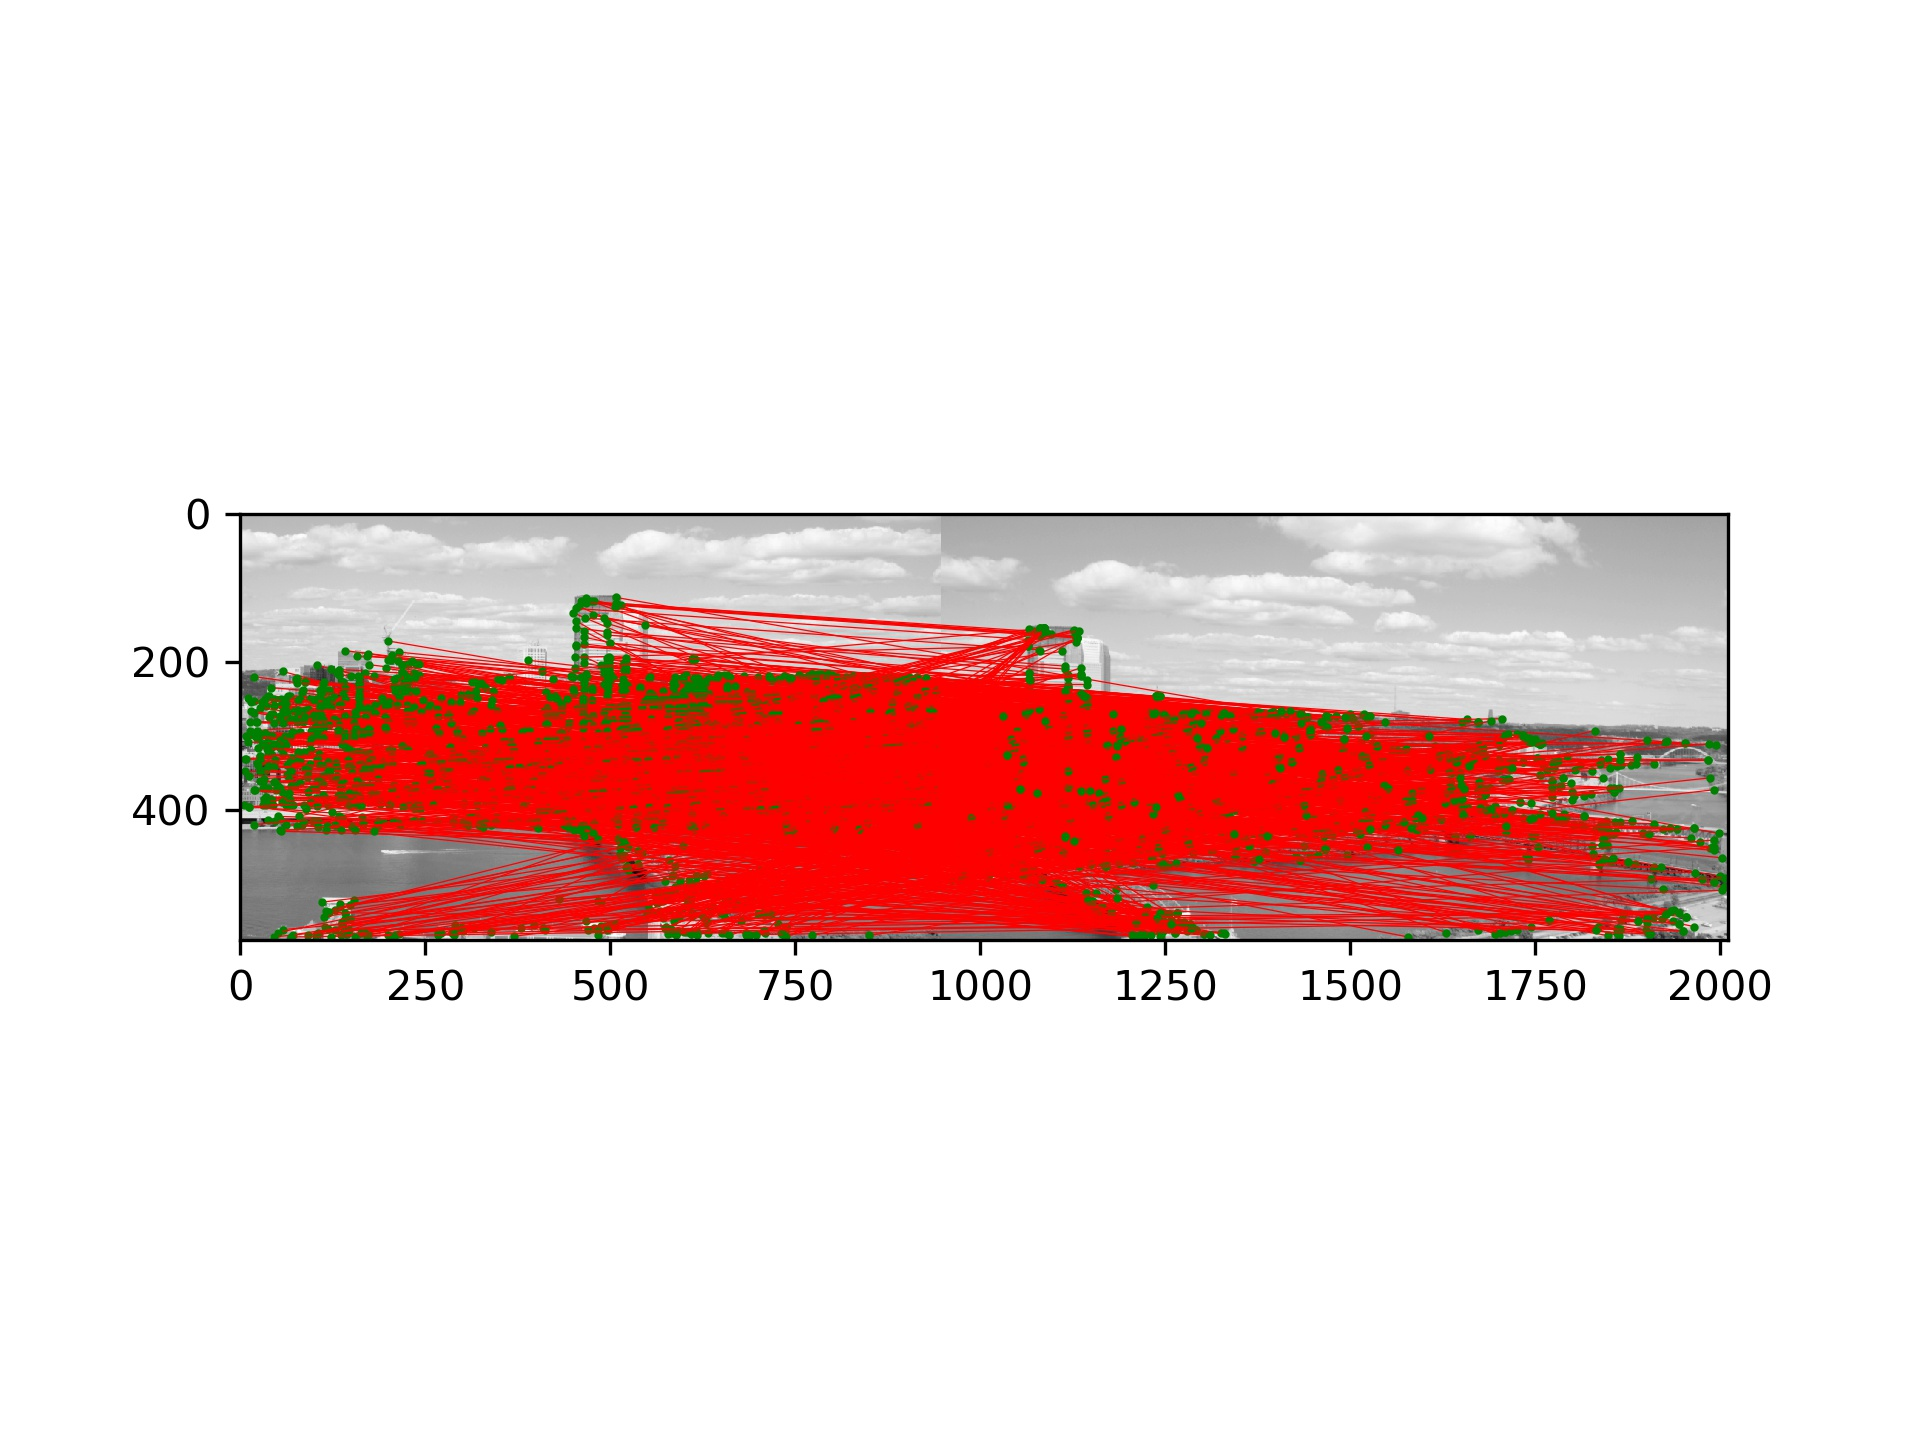
\includegraphics[width=.8\linewidth]{../results/incline_match.jpg}
      \caption{match of the \code{incline} images. }
    \end{subfigure}
    \begin{subfigure}{.327\textwidth}
      \centering
      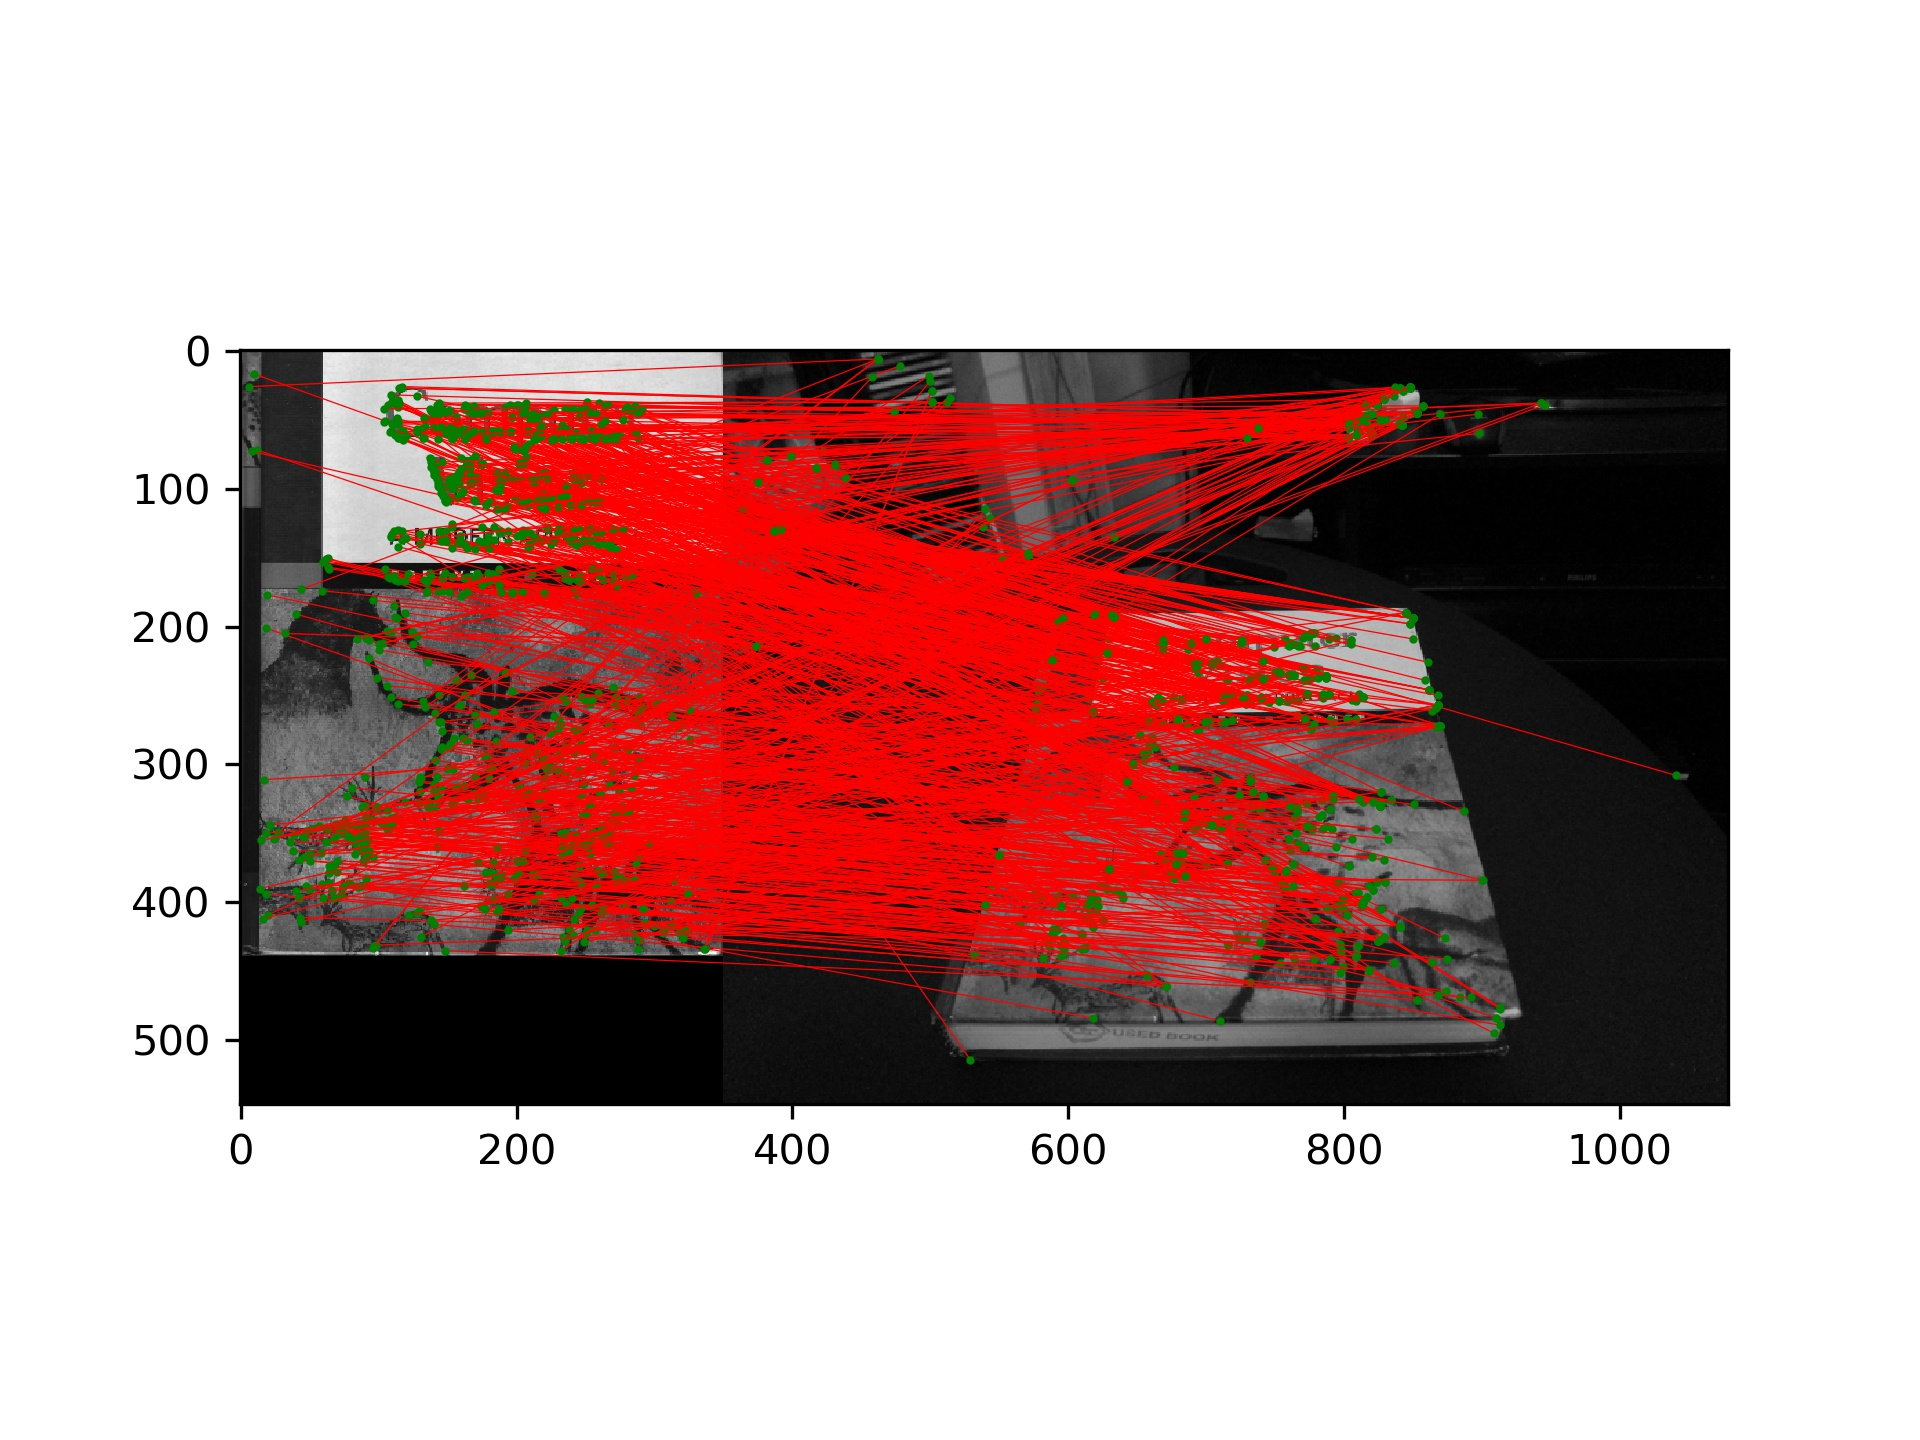
\includegraphics[width=.8\linewidth]{../results/pf_desk_match.jpg}
      \caption{match of \code{pf\_scan\_scaled.jpg} against \code{pf\_desk.jpg}.}
    \end{subfigure}
    \begin{subfigure}{.327\textwidth}
      \centering
      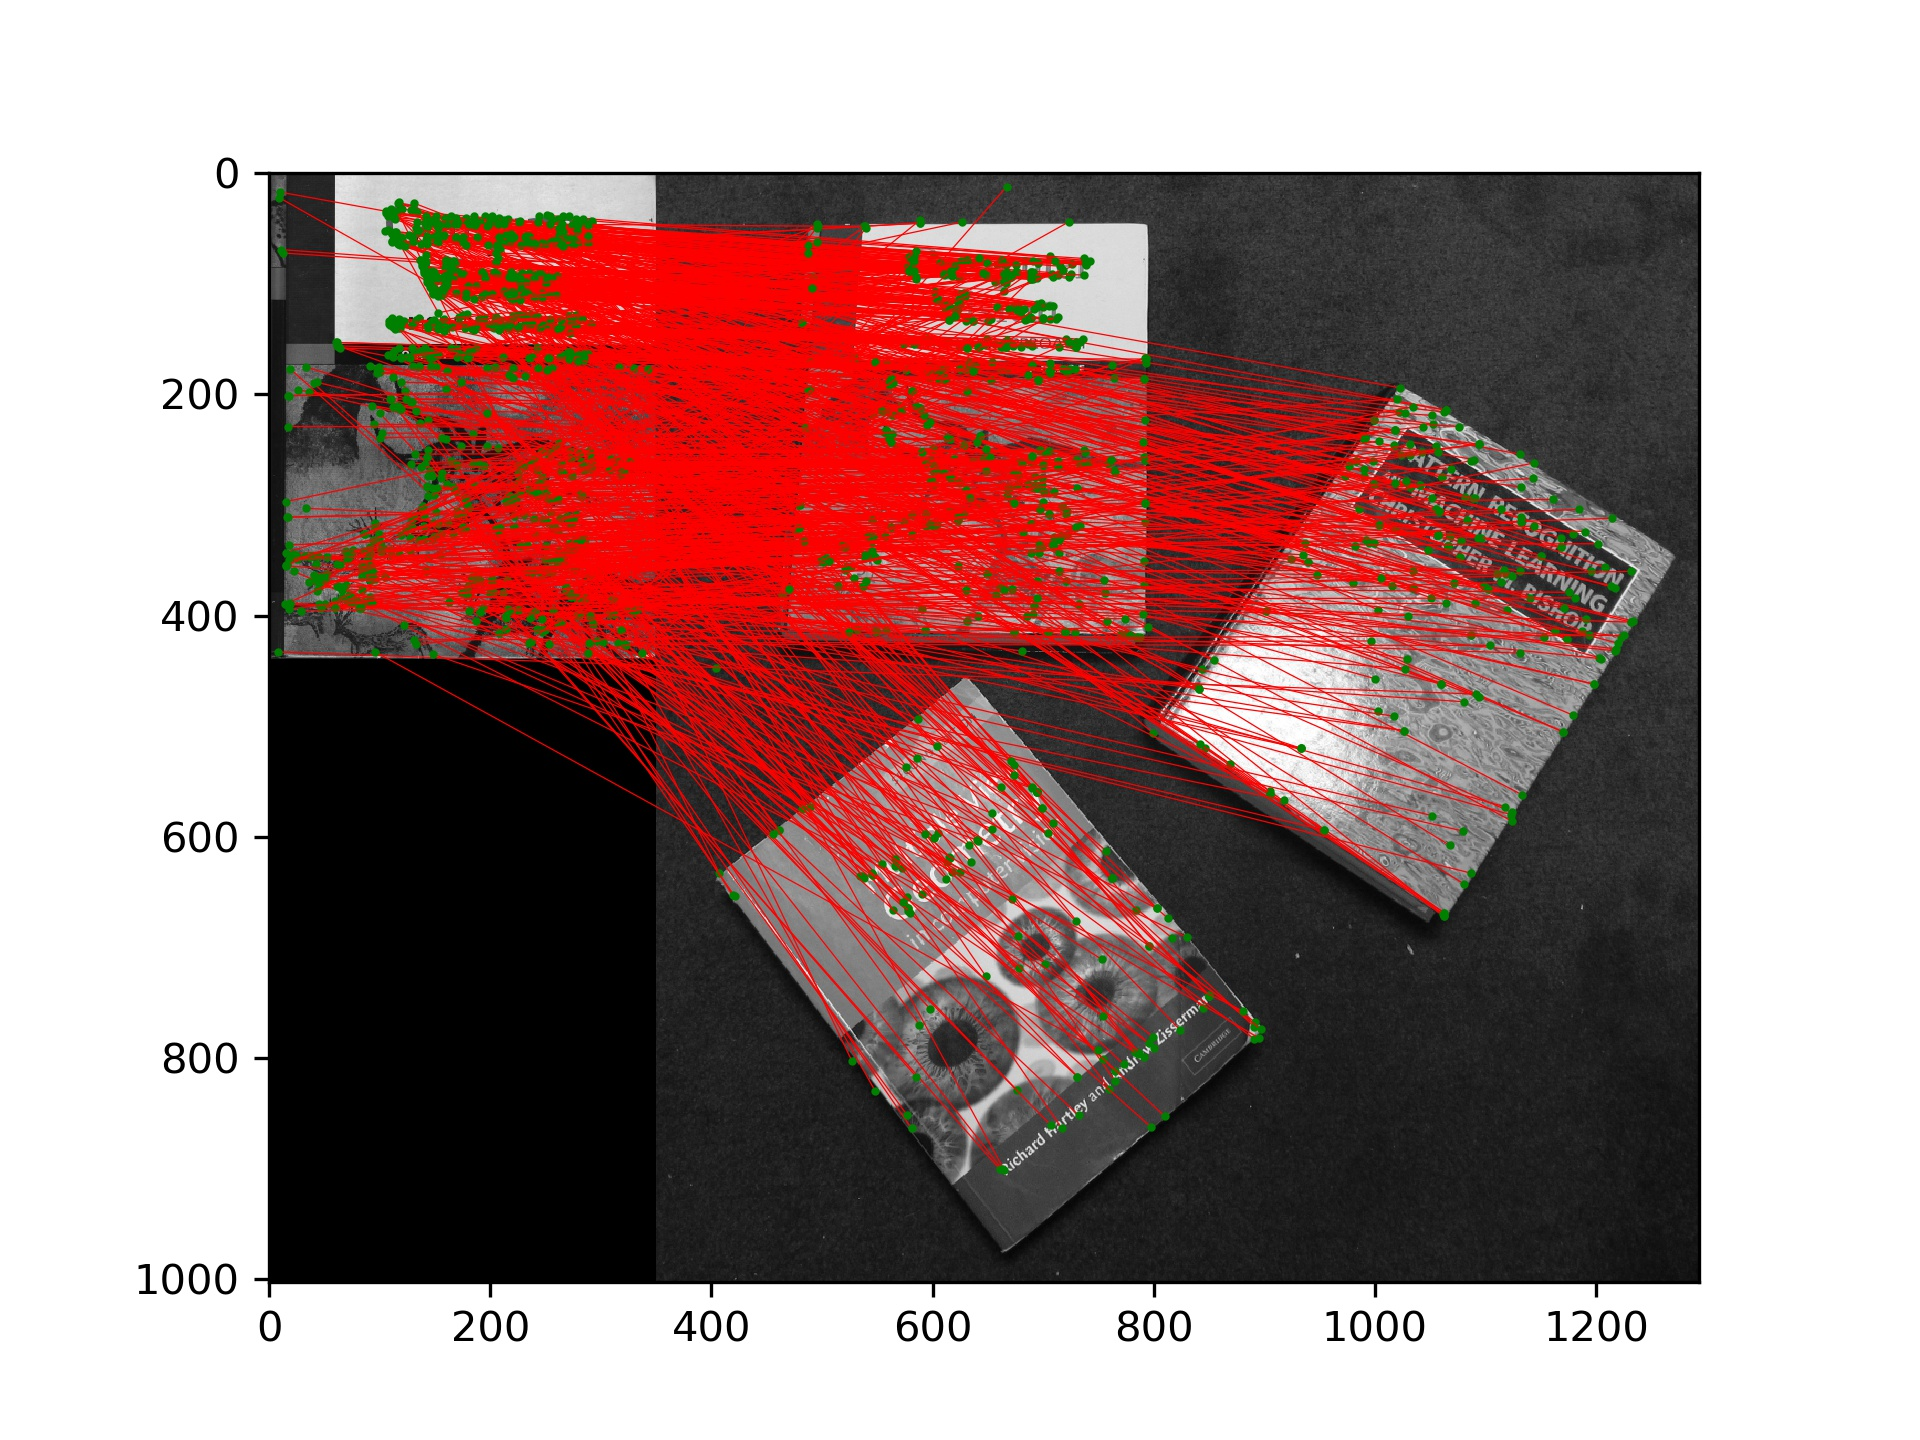
\includegraphics[width=.8\linewidth]{../results/pf_floor_match.jpg}
      \caption{match of \code{pf\_scan\_scaled.jpg} against \code{pf\_floor.jpg}.}
    \end{subfigure}
    \begin{subfigure}{.327\textwidth}
      \centering
      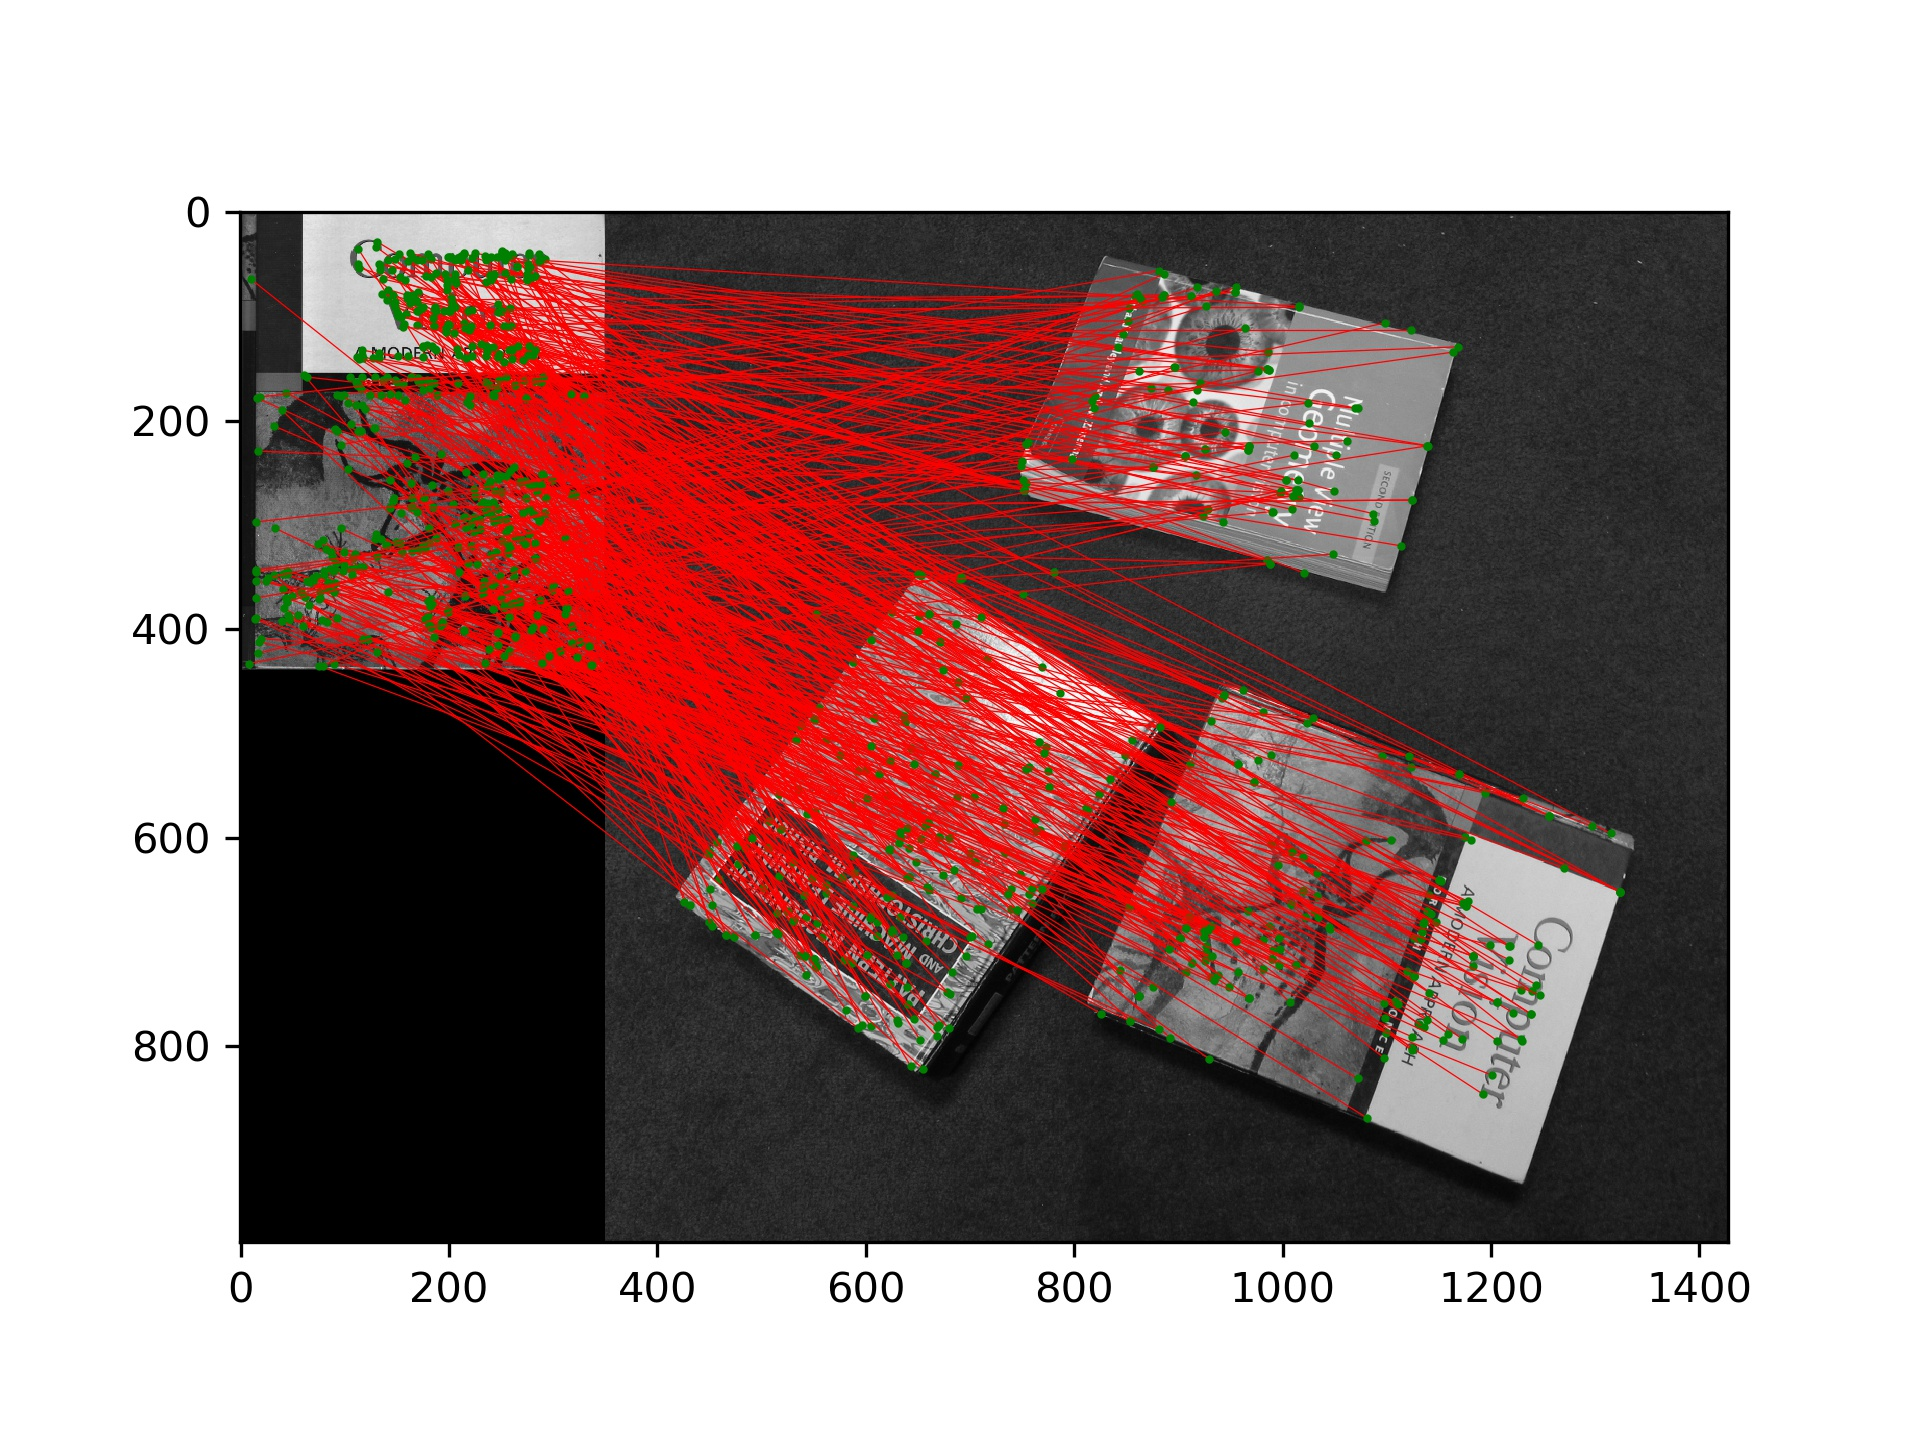
\includegraphics[width=.8\linewidth]{../results/pf_floor_rot_match.jpg}
      \caption{match of \code{pf\_scan\_scaled.jpg} against \code{pf\_floor\_rot.jpg}.}
    \end{subfigure}
    \begin{subfigure}{.327\textwidth}
      \centering
      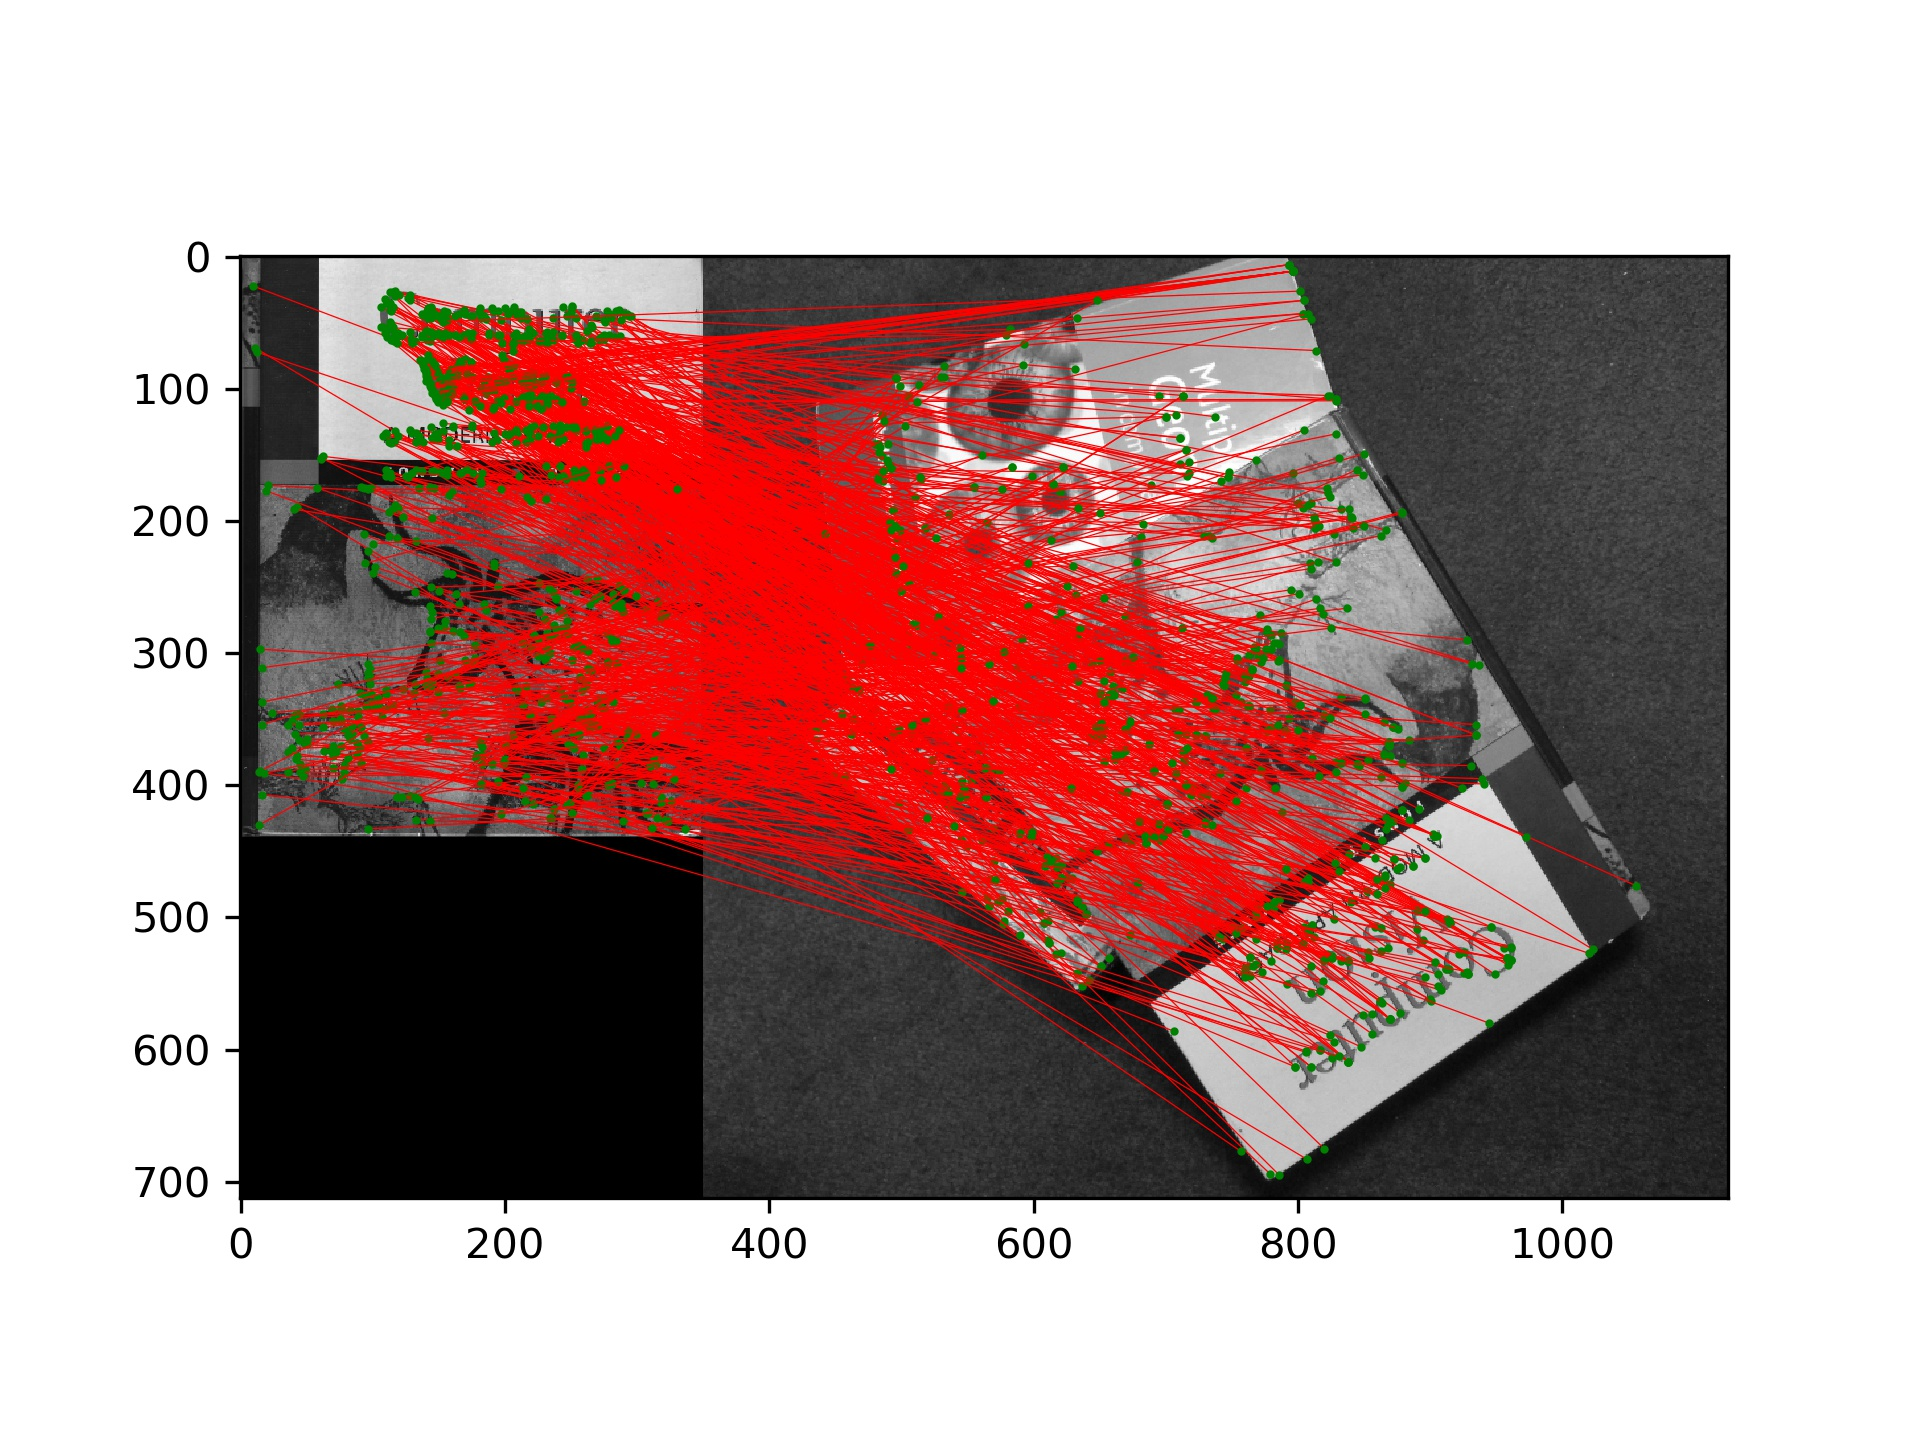
\includegraphics[width=.8\linewidth]{../results/pf_pile_match.jpg}
      \caption{match of \code{pf\_scan\_scaled.jpg} against \code{pf\_pile.jpg}.}
    \end{subfigure}
    \begin{subfigure}{.327\textwidth}
      \centering
      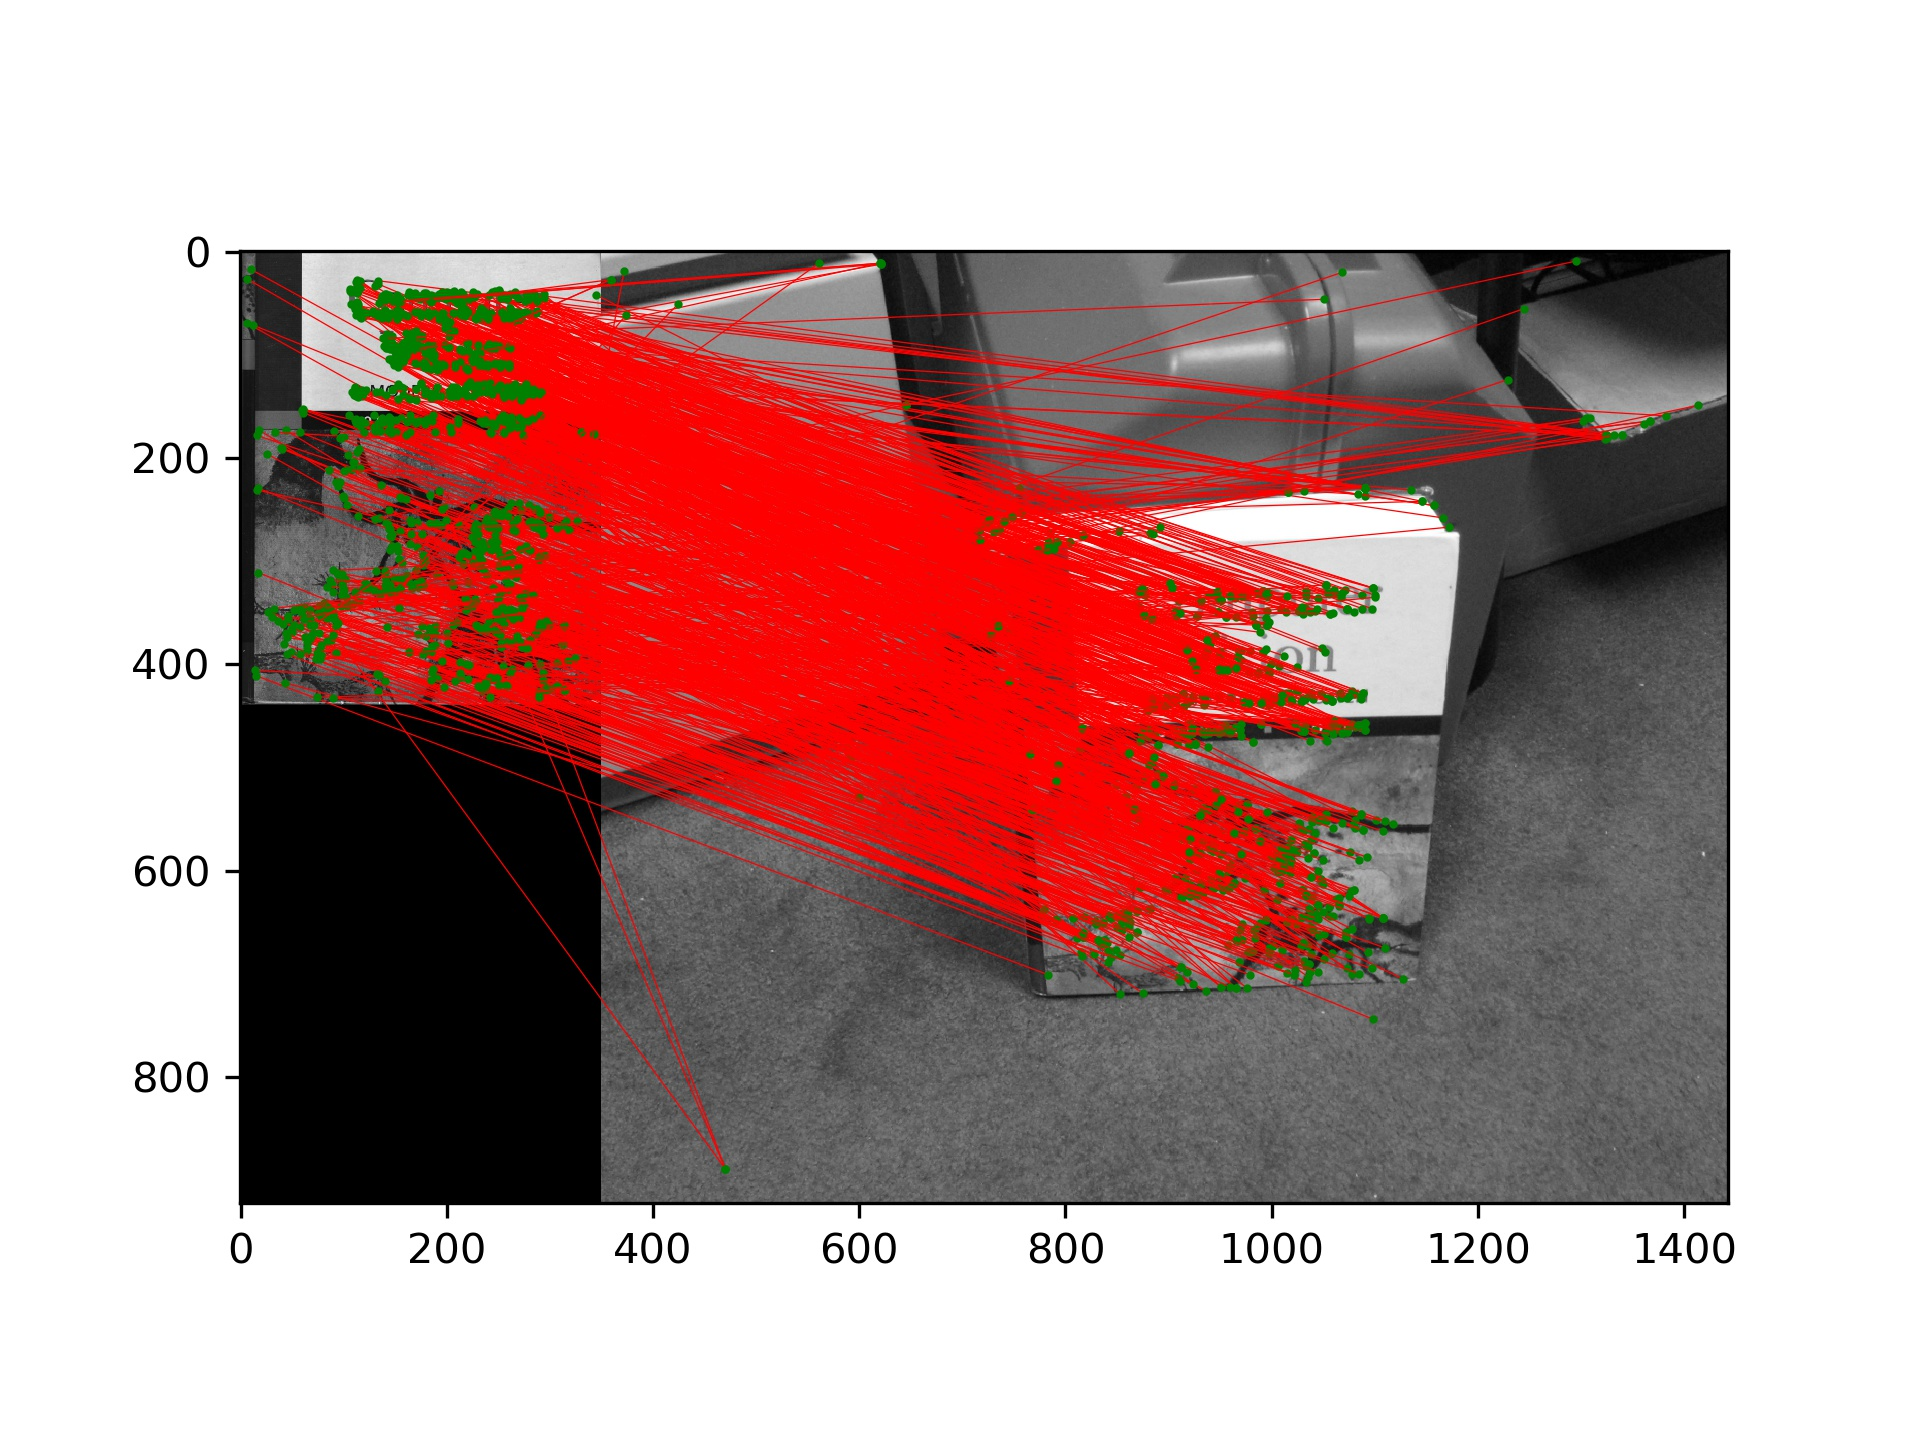
\includegraphics[width=.8\linewidth]{../results/pf_stand_match.jpg}
      \caption{match of \code{pf\_scan\_scaled.jpg} against \code{pf\_stand.jpg}.}
    \end{subfigure}
    \caption{Results of Feature Match. }
    \label{fig:q2.4}
\end{figure}

\newpage

\subsection*{Q2.5}

Please see Figure~\ref{fig:q2.5} for the matching results. As we can see, the number of matches reaches its maximum when there is no rotation between two images, and drops quickly when the rotation angle starts to increase. This is probably because the BRIEF descriptor we Implement only treats each keypoint patch as a rectangle grid, and thus when the rectangle is rotated, the whole grid structure can be messed up. Therefore the number of matches drops quickly as with rotation.

\begin{figure}[h!]
    \centering
    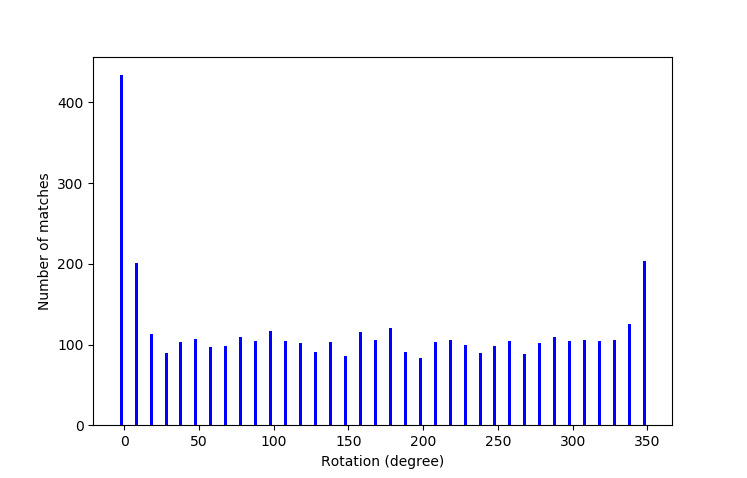
\includegraphics[width=.8\linewidth]{../results/q2_5.png}
    \caption{The rotation angle vs the number of correct matches}
    \label{fig:q2.5}
\end{figure}

\newpage

\subsection*{Q3.1}




\end{document}
